\documentclass{article}
\usepackage{lipsum}
\usepackage{braket}
\usepackage{mathrsfs}
\usepackage{amsmath}
\usepackage{graphicx}
\usepackage{listings}

\begin{document}
\title{Assignment 1}
\author{
    Name:\underline{Wang Dingrui}
}
\maketitle


\section{Program output}
The output of the program is in the figure below. 
\begin{figure}[h]
    \centering
    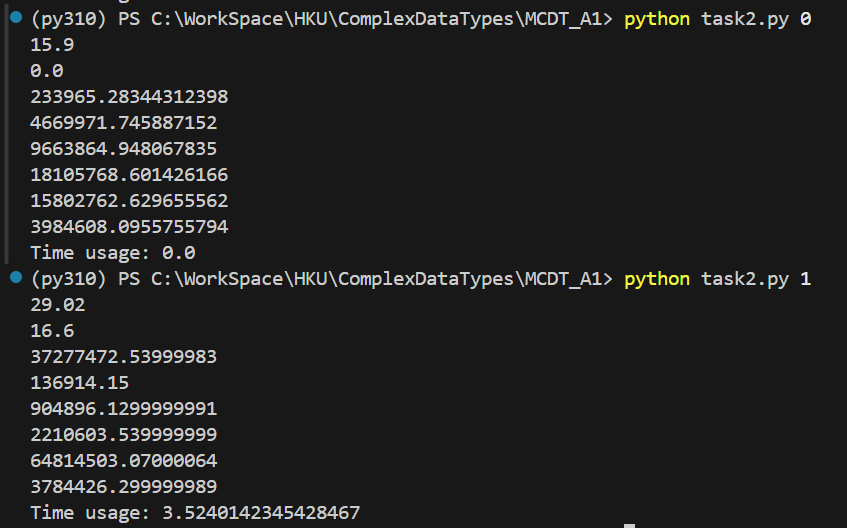
\includegraphics[width=0.8\textwidth]{out.png} % Ensure this path is correct
    \caption{Output of the program}
\end{figure}


It can be seen from the figure that approximate search has a different output from exact search.

\section{Time comparison}
I also ran the O(m*n) (m for query number and n for record number) grogram to get the ground truth. This program took approximately 160 seconds to run on intel core i5 13490F, when approximate search took 0 seconds and exact search took 3.5 seconds.

The ground truth is shown in the figure below.
\begin{figure}[h]
    \centering
    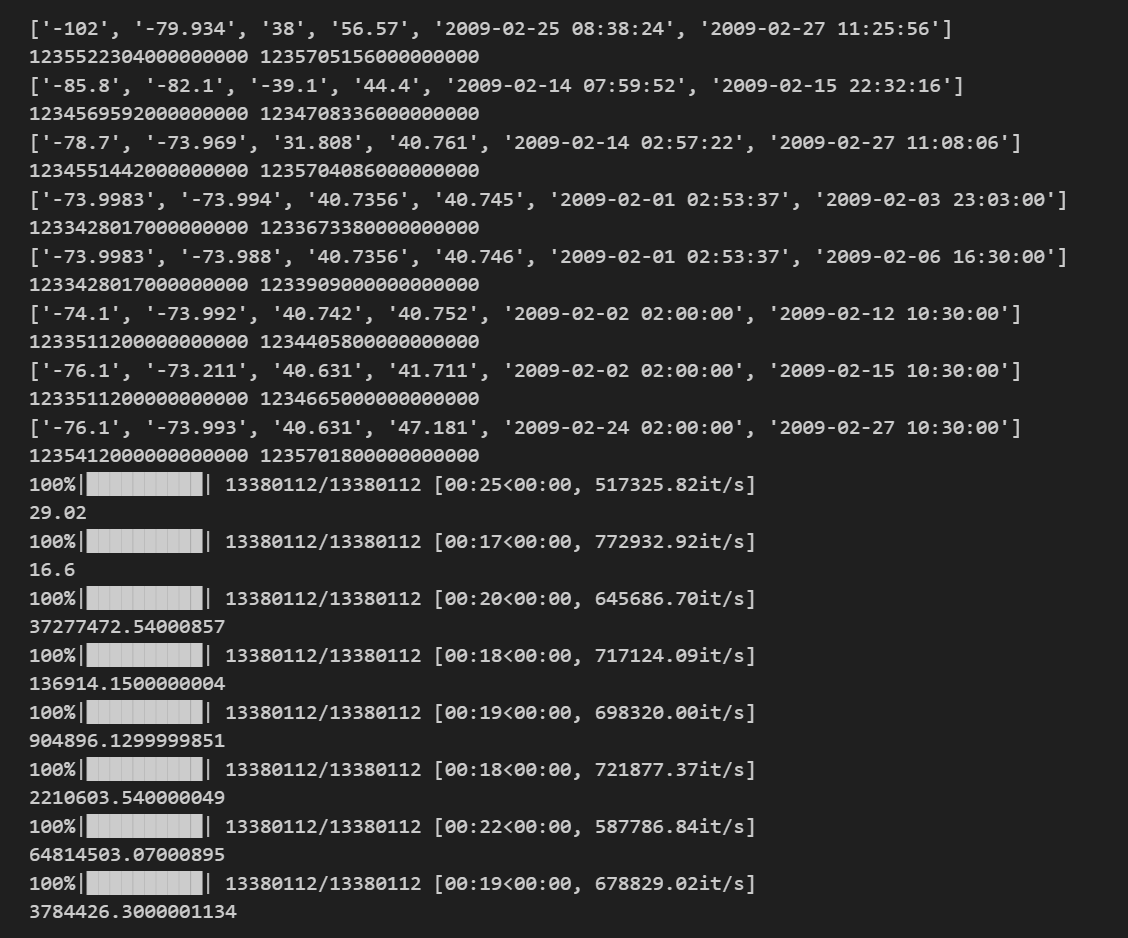
\includegraphics[width=0.8\textwidth]{gt.png} % Ensure this path is correct
    \caption{Ground truth}
\end{figure}

It can be seen that approximate search is much faster than exact search, however, the result is not as accurate as exact search.

The exact seach has the same result as the ground truth, it is much faster than the O(m*n) program. This shows that building an index is very important for large scale data, and grid index is a good choice for 3D data.

\section{Code}
\subsection{How to run the code}
My development environment is python 3.10. To run the code, you need to install the following packages:
pandas, tqdm. You can install them by running the following command:
\begin{lstlisting}[language=bash]
    pip install pandas tqdm
\end{lstlisting}

If you want to run the code, you can run the following command:
\begin{lstlisting}[language=bash]
    python task2.py 1
    python task2.py 0
\end{lstlisting}

If the argument is 1, the program will run the exact search, if the argument is 0, the program will run the approximate search.

\subsection{Code and explanation}
\begin{lstlisting}[language=Python, caption=Task 1, label=task1, breaklines=true]
    import pandas as pd
    from  tqdm import tqdm
    yellow_tripdata = pd.read_parquet('yellow_tripdata_2009-02.parquet')
    intresting_cols = ["Trip_Pickup_DateTime", "Start_Lon", "Start_Lat","Total_Amt"]
    
    intresting_data = yellow_tripdata[intresting_cols].dropna()
    
    # delete the rows with lon not in the range of [-180, 180] and lat not in the range of [-90, 90]
    # intresting_data = intresting_data[(intresting_data["Start_Lon"] >= -180) & (intresting_data["Start_Lon"] <= 180) & (intresting_data["Start_Lat"] >= -90) & (intresting_data["Start_Lat"] <= 90)]
    
    min_start_lon = intresting_data["Start_Lon"].min()
    
    max_start_lon = intresting_data["Start_Lon"].max()
    
    min_start_lat = intresting_data["Start_Lat"].min()
    
    max_start_lat = intresting_data["Start_Lat"].max()
    
    #convert the date time to datetime object, and get the timestamp
    intresting_data["Trip_Pickup_DateTime"] = pd.to_datetime(intresting_data["Trip_Pickup_DateTime"])
    
    min_trip_pickup_datetime = intresting_data["Trip_Pickup_DateTime"].min().value
    
    max_trip_pickup_datetime = intresting_data["Trip_Pickup_DateTime"].max().value
    
    # print(min_start_lon, max_start_lon, min_start_lat, max_start_lat, min_trip_pickup_datetime, max_trip_pickup_datetime)
    
    def get_grid_loc(time, lon, lat, min_time = min_trip_pickup_datetime, max_time = max_trip_pickup_datetime, min_lon = min_start_lon, max_lon = max_start_lon, min_lat = min_start_lat, max_lat = max_start_lat, grid_size = 100):
        time_loc = int((time.value - min_time)/(max_time - min_time+0.000001)*grid_size)
        lon_loc = int((lon - min_lon)/(max_lon - min_lon+0.000001)*grid_size)
        lat_loc = int((lat - min_lat)/(max_lat - min_lat+0.000001)*grid_size)
        time_loc = time_loc - 1 if time_loc != 0 else 0
        lon_loc = lon_loc - 1 if lon_loc != 0 else 0
        lat_loc = lat_loc - 1 if lat_loc != 0 else 0
        return (lon_loc, lat_loc, time_loc)
        
    
    grid = [[[[] for i in range(100)] for j in range(100)] for k in range(100)]
    
    for index, row in tqdm(intresting_data.iterrows(),total=intresting_data.shape[0]):
        grid_loc = get_grid_loc(row["Trip_Pickup_DateTime"], row["Start_Lon"], row["Start_Lat"])
        grid[grid_loc[0]][grid_loc[1]][grid_loc[2]].append((row["Start_Lon"], row["Start_Lat"],row["Trip_Pickup_DateTime"].value, row["Total_Amt"]))
        
        
    
        
        
        
    with open("grid.txt", "w") as f:
        header = f"""{min_start_lon}, {max_start_lon}\n{min_start_lat}, {max_start_lat}\n{min_trip_pickup_datetime}, {max_trip_pickup_datetime}\n"""
        f.write(header)
        for i in range(100):
            for j in range(100):
                for k in range(100):
                    f.write(f"({i},{j},{k})\n")
                    total = sum([l[3] for l in grid[i][j][k]])
                    print(total,[l[3] for l in grid[i][j][k]])
                    f.write(f"{total}\n")
                    for l in grid[i][j][k]:
                        f.write(f"{l[0]},{l[1]},{l[2]},{l[3]}\n")
                        
                        
\end{lstlisting}


In this code, I first read the data from the parquet file, 
and then got the interesting columns. 
I then dropped the rows with missing values. 
After that, I got the min and max of the longitude, latitude and timestamp. 
Then, I converted the timestamp to datetime object and get the timestamp. Later I defined a function to get the grid location of a record. Lastly, I built the grid index and write it to a file.

\begin{lstlisting}[language=Python, caption=Task 2, label=task2, breaklines=true]
    from tqdm import tqdm

    with open("grid.txt") as f:
        min_start_lon,max_start_lon = map(float, f.readline().strip().split(","))
        min_start_lat,max_start_lat = map(float, f.readline().strip().split(","))
        min_trip_pickup_datetime,max_trip_pickup_datetime = map(int, f.readline().strip().split(","))
        x_unit = (max_start_lon - min_start_lon)/100
        y_unit = (max_start_lat - min_start_lat)/100
        z_unit = (max_trip_pickup_datetime - min_trip_pickup_datetime)/100
        grid_size = 100
        grid = [[[[] for i in range(100)] for j in range(100)] for k in range(100)]
        grid_total_amts = [[[0 for i in range(100)] for j in range(100)] for k in range(100)]
        lon_loc, lat_loc, time_loc = 0,0,0
        
        while s:=f.readline():
            if s.startswith("("):
                lon_loc, lat_loc, time_loc = eval(s.strip())
                Grid_Total_Amt = float(f.readline().strip())
                grid_total_amts[lon_loc][lat_loc][time_loc] = Grid_Total_Amt
            else:
                # line_s = f.readline()
                # print(line_s)
                Start_lon, Start_Lat, Trip_Pickup_DateTime,Total_Amt = s.strip().split(",")
                
                Start_lon = float(Start_lon)
                Start_Lat = float(Start_Lat)
                Trip_Pickup_DateTime = int(Trip_Pickup_DateTime)
                Total_Amt = float(Total_Amt)
                # print(Start_Lat, Start_lon, Trip_Pickup_DateTime, Total_Amt)
                grid[lon_loc][lat_loc][time_loc].append((Start_lon, Start_Lat, Trip_Pickup_DateTime, Total_Amt))
                
    from datetime import datetime
    def query_text_to_list(s):
        query_str_list = s.strip().split(",")
        low_x = float(query_str_list[0])
        up_x = float(query_str_list[1])
        low_y = float(query_str_list[2])
        up_y = float(query_str_list[3])
        low_time = int(datetime.strptime(query_str_list[4], "%Y-%m-%d %H:%M:%S").timestamp())*1000000000
        up_time = int(datetime.strptime(query_str_list[5], "%Y-%m-%d %H:%M:%S").timestamp())*1000000000
        # print(query_str_list)
        # print(low_time, up_time)
        return [low_x, up_x, low_y, up_y, low_time, up_time]
        
    
    with open("queries.txt") as f:
        queries = f.readlines()
        struc_queries = list(map(query_text_to_list, queries))
    
    
    
    def get_grid_loc(time, lon, lat, min_time = min_trip_pickup_datetime, max_time = max_trip_pickup_datetime, min_lon = min_start_lon, max_lon = max_start_lon, min_lat = min_start_lat, max_lat = max_start_lat, grid_size = 100):
        time_loc = int((time - min_time)/(max_time - min_time+0.000001)*grid_size)
        lon_loc = int((lon - min_lon)/(max_lon - min_lon+0.000001)*grid_size)
        lat_loc = int((lat - min_lat)/(max_lat - min_lat+0.000001)*grid_size)
        time_loc = time_loc - 1 if time_loc != 0 else 0
        lon_loc = lon_loc - 1 if lon_loc != 0 else 0
        lat_loc = lat_loc - 1 if lat_loc != 0 else 0
        return (lon_loc, lat_loc, time_loc)
    
    
    def calc_fraction(i,j,k, low_x, up_x, low_y, up_y, low_time, up_time,):
        min_x = min_start_lon + (max_start_lon - min_start_lon)/100*i
        max_x = min_start_lon + (max_start_lon - min_start_lon)/100*(i+1)
        min_y = min_start_lat + (max_start_lat - min_start_lat)/100*j
        max_y = min_start_lat + (max_start_lat - min_start_lat)/100*(j+1)
        min_time = min_trip_pickup_datetime + (max_trip_pickup_datetime - min_trip_pickup_datetime)/100*k
        max_time = min_trip_pickup_datetime + (max_trip_pickup_datetime - min_trip_pickup_datetime)/100*(k+1)
        
        intersection = (min(max_x, up_x) - max(min_x, low_x)) * (min(max_y, up_y) - max(min_y, low_y)) * (min(max_time, up_time) - max(min_time, low_time))
        
        box_vol = (max_x - min_x) * (max_y - min_y) * (max_time - min_time)
        
        # print(intersection, box_vol)
        fraction = intersection/box_vol
        # print(fraction)
        
        
        # if min_x<low_x:
        #     x_per = (max_x - low_x)/(max_x - min_x)
    
        # else:
        #     x_per = (up_x - min_x)/(max_x - min_x)
        # x_per = max(0, x_per)
        # x_per = min(1, x_per)
        # if min_y<low_y:
        #     y_per = (max_y - low_y)/(max_y - min_y)
        # else:
        #     y_per = (up_y - min_y)/(max_y - min_y)
        # y_per = max(0, y_per)
        # y_per = min(1, y_per)
        # if min_time<low_time:
        #     time_per = (max_time - low_time)/(max_time - min_time)
        # else:
        #     time_per = (up_time - min_time)/(max_time - min_time)
        # time_per = max(0, time_per)
        # time_per = min(1, time_per)
        # print("x_max:", max_x, "x_min:", min_x, "y_max:", max_y, "y_min:", min_y, "time_max:", max_time, "time_min:", min_time)
        # print("x_up:", up_x, "x_low:", low_x, "y_up:", up_y, "y_low:", low_y, "time_up:", up_time, "time_low:", low_time)
        # print(x_per, y_per, time_per), abs(x_per*y_per*time_per)
        # return abs(x_per*y_per*time_per)
        return max(0, fraction)
    
    
    class Query:
        def __init__(self, low_x, up_x, low_y, up_y, low_time, up_time):
            self.low_x = low_x
            self.up_x = up_x
            self.low_y = low_y
            self.up_y = up_y
            self.low_time = low_time
            self.up_time = up_time
            self.low_x_grid, self.low_y_grid, self.low_time_grid = get_grid_loc(low_time, low_x, low_y)
            self.up_x_grid, self.up_y_grid, self.up_time_grid = get_grid_loc(up_time, up_x, up_y)
            # low_x_grid = int((self.low_time - min_trip_pickup_datetime)/(max_trip_pickup_datetime - min_trip_pickup_datetime+0.000001)*grid_size)
            # up_x_grid = int((self.up_time - min_trip_pickup_datetime)/(max_trip_pickup_datetime - min_trip_pickup_datetime+0.000001)*grid_size)
            # low_y_grid = int((self.low_x - min_start_lon)/(max_start_lon - min_start_lon+0.000001)*grid_size)
            # up_y_grid = int((self.up_x - min_start_lon)/(max_start_lon - min_start_lon+0.000001)*grid_size)
            # low_time_grid = int((self.low_y - min_start_lat)/(max_start_lat - min_start_lat+0.000001)*grid_size)
            # up_time_grid = int((self.up_y - min_start_lat)/(max_start_lat - min_start_lat+0.000001)*grid_size)
            # self.low_x_grid = low_x_grid - 1 if low_x_grid != 0 else 0
            # self.up_x_grid = up_x_grid - 1 if up_x_grid != 0 else 0
            # self.low_y_grid = low_y_grid - 1 if low_y_grid != 0 else 0
            # self.up_y_grid = up_y_grid - 1 if up_y_grid != 0 else 0
            # self.low_time_grid = low_time_grid - 1 if low_time_grid != 0 else 0
            # self.up_time_grid = up_time_grid - 1 if up_time_grid != 0 else 0
        def get_low_x_grid(self):
            return self.low_x_grid
        def get_up_x_grid(self):
            return self.up_x_grid
        def get_low_y_grid(self):
            return self.low_y_grid
        def get_up_y_grid(self):
            return self.up_y_grid
        def get_low_time_grid(self):
            return self.low_time_grid
        def get_sum_grid_points_in_query(self,grid_points):
            # print(grid_points)
            sum = 0
            for grid_point in grid_points:
                if grid_point[0] >= self.low_x and grid_point[0] <= self.up_x and grid_point[1] >= self.low_y and grid_point[1] <= self.up_y and grid_point[2] >= self.low_time and grid_point[2] <= self.up_time:
                    sum+=grid_point[3]
            return sum
        def exac_query(self):
            sum = 0
            # print(self.low_x_grid, self.up_x_grid, self.low_y_grid, self.up_y_grid, self.low_time_grid, self.up_time_grid)
            for i in range(self.low_x_grid, self.up_x_grid+1):
                for j in range(self.low_y_grid, self.up_y_grid+1):
                    for k in range(self.low_time_grid, self.up_time_grid+1):
                        if i == self.low_x_grid or i == self.up_x_grid or j == self.low_y_grid or j == self.up_y_grid or k == self.low_time_grid or k == self.up_time_grid:
                            sum+=self.get_sum_grid_points_in_query(grid[i][j][k])
                        else:
                            sum += grid_total_amts[i][j][k]
            return sum
        def approx_query(self):
            sum = 0
            # print(self.low_x_grid, self.up_x_grid, self.low_y_grid, self.up_y_grid, self.low_time_grid, self.up_time_grid)
            for i in range(self.low_x_grid, self.up_x_grid+1):
                for j in range(self.low_y_grid, self.up_y_grid+1):
                    for k in range(self.low_time_grid, self.up_time_grid+1):
                        if i == self.low_x_grid or i == self.up_x_grid or j == self.low_y_grid or j == self.up_y_grid or k == self.low_time_grid or k == self.up_time_grid:
                            sum += calc_fraction(i,j,k, self.low_x, self.up_x, self.low_y, self.up_y, self.low_time, self.up_time)*grid_total_amts[i][j][k]
                        else:
                            sum += grid_total_amts[i][j][k]
            return sum
        
    
    if __name__ == "__main__":
        import sys
        exact = int(sys.argv[1])
        from time import time
        start = time()
        if exact == 0:
            for query in struc_queries:
                query = Query(*query)
                print(query.approx_query())
        elif exact == 1:
            for query in struc_queries:
                query = Query(*query)
                print(query.exac_query())
        else:
            for query in struc_queries:
                query = Query(*query)
                print(query.exac_query())
                print(query.approx_query())
                print()
        print("Time usage:",time()-start)
    
        # with open("exact_results1.txt", "w") as f:
        #     for query in tqdm(struc_queries):
        #         query = Query(*query)
        #         # print(query.exac_query())
        #         f.write(str(query.exac_query()) + "\n")
                
        # with open("approx_results1.txt", "w") as f:
        #     for query in tqdm(struc_queries):
        #         query = Query(*query)
        #         # print(query.approx_query())
        #         f.write(str(query.approx_query()) + "\n")
            
\end{lstlisting}


In task2.py, I wrote a class Query to represent a query. 
Then, I wrote a function to convert the query text to a list. 
Later, I read the grid index from the file and build the grid index. 
After that, I read the queries from the file and convert them to a list. 
Also, I wrote a function to calculate the fraction of the intersection of the query box and the grid box.
Then, I wrote a class Query to represent a query. 
A function is wrotten to calculate the exact query result and the approximate query result. Lastly, I wrote the main function to run the queries and print the results. I also wrote the code to write the results to a file.


\end{document}